\documentclass[11pt]{article}
\usepackage[a4paper, hmargin={2.5cm, 2.5cm}, vmargin={2.5cm, 2.5cm}]{geometry}
\usepackage{eso-pic} % \AddToShipoutPicture
\usepackage{graphicx} % \includegraphics
\usepackage{amsmath}
\usepackage{amsfonts}
\usepackage{amssymb}
\usepackage{graphicx}
\usepackage{fancyhdr}
\usepackage{moreverb}
\usepackage{lscape}
\usepackage[utf8]{inputenc}
\usepackage{caption}
\usepackage{subcaption}
\usepackage{float}


% Ved at bruge kommandoen \newcommand kan man forkorte kommandoer eller ændre dem til noget mere passende.
\newcommand{\setR}{\mathbb{R}}
\newcommand{\setZ}{\mathbb{Z}}
\newcommand{\setN}{\mathbb{N}}
\newcommand{\setF}{\mathbb{F}}
\newcommand{\lra}{\Leftrightarrow}
\newcommand{\ra}{\Rightarrow}
\newcommand{\ac}{\textasciicircum}
\newcommand{\uuline}[1]{\underline{\underline{#1}}}
\newcommand{\bpm}{\begin{pmatrix}}
\newcommand{\epm}{\end{pmatrix}}

\renewcommand{\headrulewidth}{0pt}

\author{Thomas Nyegaard-Signori\\
  Enes Golic\\
  Tor-Salve Dalsgaard\\
  Tobias Carlos Tvarnø
  \Large{}
  \\ \texttt{} \\
}

\title{Mobile computing - Hololens and LEGO
  \vspace{3cm}
  \Huge{} \\
  \Large{}
}

\begin{document}

%% Change `ku-farve` to `nat-farve` to use SCIENCE's old colors or
%% `natbio-farve` to use SCIENCE's new colors and logo.
\AddToShipoutPicture*{\put(0,0){\includegraphics*[viewport=0 0 700 600]{include/ku-farve}}}
\AddToShipoutPicture*{\put(0,602){\includegraphics*[viewport=0 600 700 1600]{include/ku-farve}}}

%% Change `ku-en` to `nat-en` to use the `Faculty of Science` header
\AddToShipoutPicture*{\put(0,0){\includegraphics*{include/ku-en}}}

\clearpage\maketitle
\thispagestyle{empty}

\newpage

% !TeX root = ../project.tex

\section{Introduction}
This report focuses on an application for the newly released Microsoft Hololens. The Hololens was released around march 2017, and the fact that the product is in its infant stage and is based on a very new technology opens up possibilities and removes any preconceived notions about which applications and uses the Hololens might have.\\
The technology is relevant with regards to mobile computing in one very apparent way, in that it is a wearable, computing unit. Other than that, it offers alternate reality (AR) possibilities because of its partly see-through screens and user tracking. Since the Hololens is still a new technology, the mobility and computing power of the product will most likely increase, making it resemble a ubiquitous computer more and more. This evolution of mobile computing was one of the reasons that the Hololens was chosen to develop on in the first place.\\\\
The application this report will cover revolves around LEGO. LEGO is a way for kids and adults to build constructions, vehicles and scenery, all in a very physical and three-dimensional way. This, then, seemed like a natural choice for an AR application, since the application layer between the user and the world could expand naturally on the possibilities and limitations of the physical, "real-world" LEGO.\\
The application in itself should be a sort of digital playground in which a user could interact with LEGO in ways they would find natural. Sticking pieces together the way they do in real life, stacking and constructing, all interactions that the user knows well from having played around with real LEGO. This was done using interaction through a virtual tablet, known as the "Generator board" and simple drag-and-drop with the bricks. We end up with a rough prototype which helped us discover the pitfalls and consideration concerning a LEGO implementation in an AR enviroment. 

\section{Sketching}
The structure can look like this:
\begin{itemize}
	\item Present the chosen design challenges and some of the initial concerns in the beginning phase
	\item Each challenge is outlined with:
		\begin{itemize}
			\item Sketches
			\item Design thoughts for the sketch - what was the thought behind this sketch?
			\item summary of the group discussion for this case - what worked, what didn't and why?
		\end{itemize}
	\item Conclude what the final sketches are - what do they accomplish, and what do they lack(maybe reference what might be discussed in future work)?
\end{itemize}
\subsection{How do we access the application? (Menu)}
The menu is an essential part of any application. It outlines the possibilities for the user in a simple fashion. The menu is something every user has experience with, as it is the first thing a user is met with when running an application. This means that the menu has to contain of certain classic elements.\par A user needs a way to close the application. On mobile phones nowadays this can be done with 'return' buttons on the phone, but all applications generally have a built in exit function.\par
The user also needs to have some sort of options menu, and guidelines. This is a must for this application. Stacking LEGO seems simple and intuitive, but all the operations and possibilities is something that can confuse a potential user. \par
Lastly the menu needs to have an easy access to the LEGO session itself. It shouldn't be complicated for the user to start a new LEGO session, meaning that this action should be as intuitive as it gets.\par
\begin{center}
	Insert sketch 1:
\end{center}

\subsection{The main menu screen}
The initial ideas for the main menu were generated following the 'x plus x' sketch generation principle outlined in the course. In the case of the sketching done for the main menu, a '5 plus 5' scheme was used. One common theme in the sketching of the main menu was separation of the design of the menu and the interaction with the menu, and the difficulties with making that separation. In quite a few of the earlier sketches, what was being sketched was more a way of interacting with the menu rather than the design of the menu itself.\\
\\
It became apparent that the menu had to use the gestures given from Hololens, ie., the bloom gesture. Since a fixed main menu screen could lead to different problems, such as blocking precious field of view, and a menu screen fixed to the world could be forgotten and overlooked, a gesture-activated main menu was the prefered interaction.

\subsection{The generator board}
After discussing menus in the context of the Hololens, it became apparent that there was a need for a menu that could be placed and interacted with in the real world. Using the tracking capabilities of the Hololens, different designs of the so called 'generator board' came up. The main purpose of the generator board is to generate blocks that the user can then drag out of the predefined spawning space.\\
\\
The idea came up that a menu with the same look and functionality of a tablet device could make interaction natural for the user. Having the ability to pick up, move and place the menu on a surface like a table or the floor seemed like a natural way of approaching the problem. The idea can be seen in a very early sketch in figure (HVILKEN FIGUR?):\\


\begin{figure}
\centering
  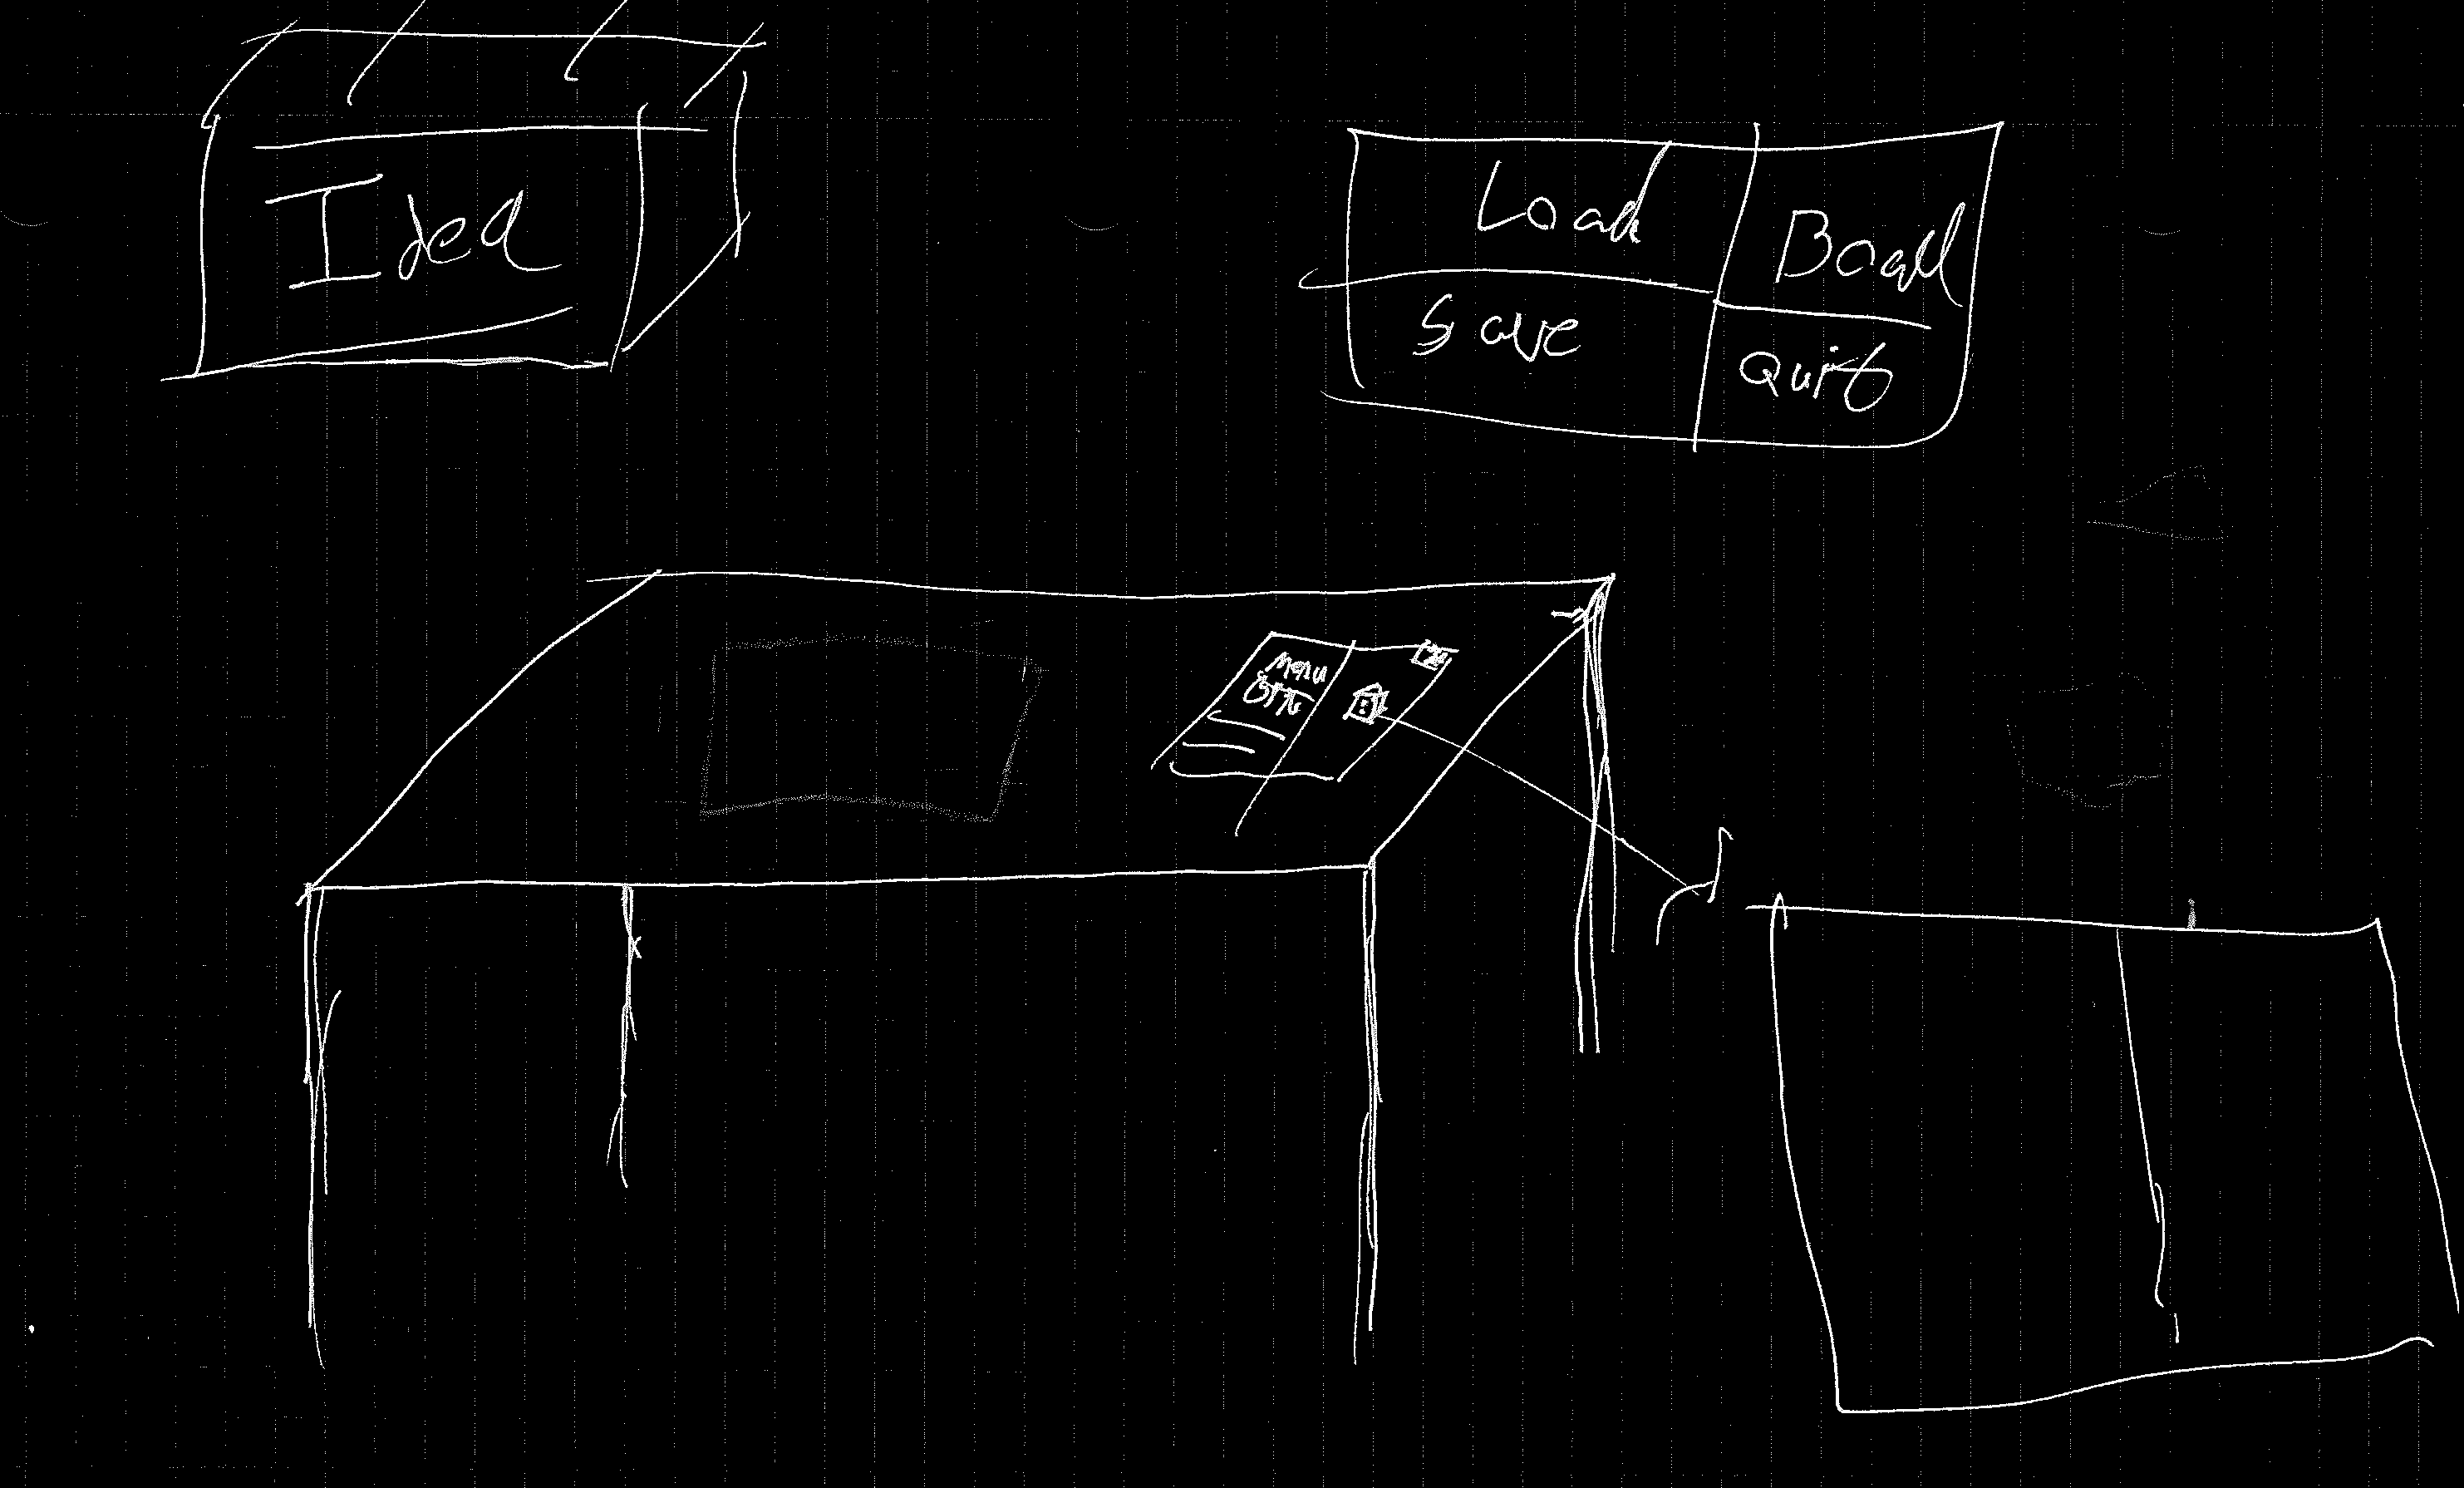
\includegraphics[width=0.9\columnwidth]{figures/Generator/gen6.png}
  \caption{Skriv lidt lækert her. }~\label{fig:genboard}
\end{figure}



\end{document}
